\begin{minipage}{.5\linewidth}
	\begin{flushleft}
		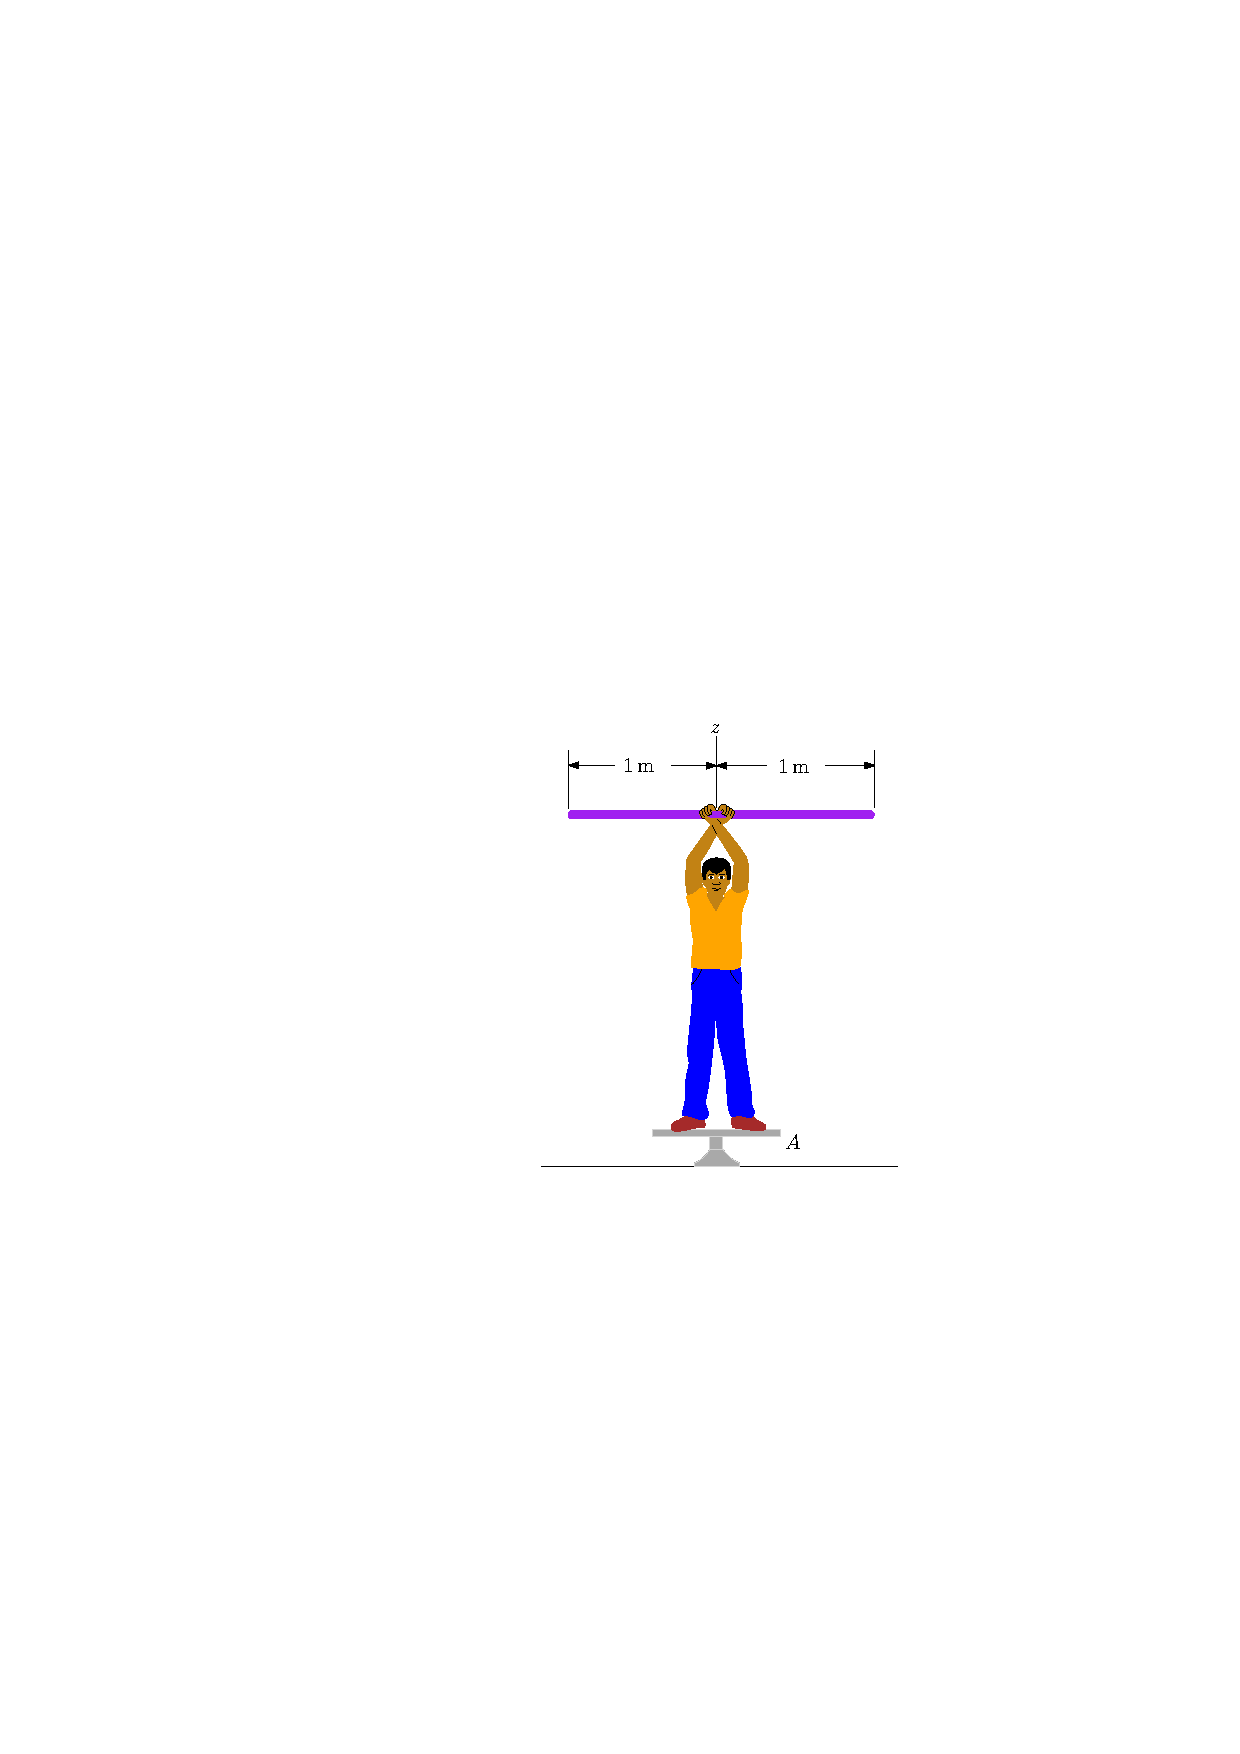
\includegraphics[scale=1.2]{../../images/draw_5}
	\end{flushleft}
\end{minipage}
\begin{minipage}{.5\linewidth}
	\item Um homem de \SI{75}{\kilogram} está parado em pé na mesa giratória $A$ e gira uma barra fina de \SI{6}{\kilogram} sobre sua cabeça. Se a velocidade angular da barra é $\omega_{r}=\SI{5}{\radian/\second}$ medida em relação ao homem e observa-se que a mesa giratória está girando na direção oposta com uma velocidade angular de $\omega_{t}=\SI{3}{\radian/\second}$, determine o raio de giração do homem em relação a seu eixo $z$. Considere a mesa giratória como um disco circular fino de raio \SI{300}{\milli\meter} e massa de \SI{5}{\kilogram}.\\
	
	\import{../answers}{answer-8}
\end{minipage}